% !TeX spellcheck = cs_CZ
%{\tikzset{external/prefix={tikz/FYZII/}}
% \tikzset{external/figure name/.add={ch10_}{}}
%---------------------------------------------------------------------------------------------------
% file fey2ch10.tex
%---------------------------------------------------------------------------------------------------
%=========================== Kapitola: Dielektrika =================================================
\setchaptertoc
\chapter{Dielektrika}\label{fyz:IIchapX}

  \section{Permitivita}\label{fyz:IIchapXsecI}
  \section{Vektor elektrické polarizace P}\label{fyz:IIchapXsecII}
  \section{Polarizační náboje}\label{fyz:IIchapXsecIII}
  \section{Elektrostatické rovnice pro dielektrika}\label{fyz:IIchapXsecIV}
  \section{Pole a síly v přítomnosti dielektrik}\label{fyz:IIchapXsecV}
  \section{Příklady a cvičení}\label{fyz:IIchapXsecVI}

    \begin{figure}[ht!] %\ref{fyz:fig705}
      \centering
      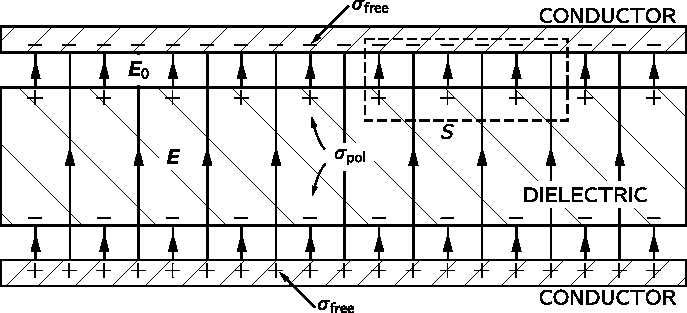
\includegraphics[width=0.9\linewidth]{fyz_fig705.pdf}
      \caption{
               (\cite[s.~707]{Feynman02})}
      \label{fyz:fig705}
    \end{figure}

    \begin{figure}[ht!] %\ref{fyz:fig706}
      \centering
      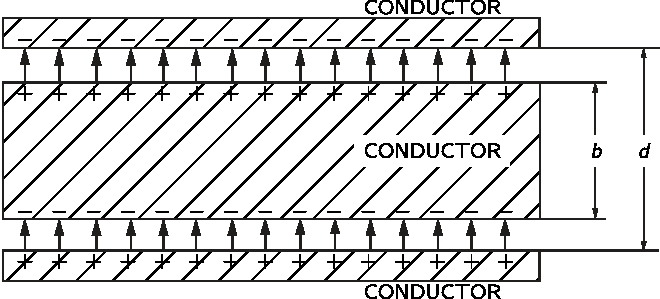
\includegraphics[width=0.9\linewidth]{fyz_fig706.pdf}
      \caption{
               (\cite[s.~707]{Feynman02})}
      \label{fyz:fig706}
    \end{figure}

    \begin{figure}[ht!] %\ref{fyz:fig707}
      \centering
      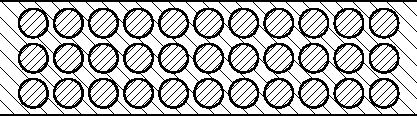
\includegraphics[width=0.9\linewidth]{fyz_fig707.pdf}
      \caption{
               (\cite[s.~707]{Feynman02})}
      \label{fyz:fig707}
    \end{figure}

    \begin{figure}[ht!]
      \centering
      \subcaptionbox{\label{fyz:fig708a}}{\luafigure[0.45]{fyz_fig708a.pdf}}
      \subcaptionbox{\label{fyz:fig708b}}{\luafigure[0.45]{fyz_fig708b.pdf}}
      \label{fyz:fig708}
      \caption{
               (\cite[s.~748]{Feynman02})}
    \end{figure}

    \begin{figure}[ht!] %\ref{fyz:fig709}
      \centering
      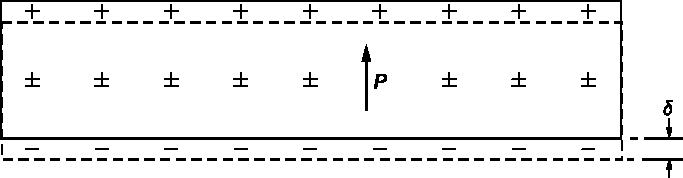
\includegraphics[width=0.5\linewidth]{fyz_fig709.pdf}
      \caption{
               (\cite[s.~707]{Feynman02})}
      \label{fyz:fig709}
    \end{figure}

    \begin{figure}[ht!] %\ref{fyz:fig710}
      \centering
      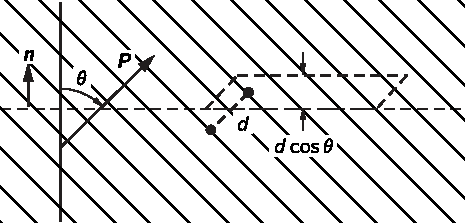
\includegraphics[width=0.5\linewidth]{fyz_fig710.pdf}
      \caption{
               (\cite[s.~707]{Feynman02})}
      \label{fyz:fig710}
    \end{figure}

    \begin{figure}[ht!] %\ref{fyz:fig711}
      \centering
      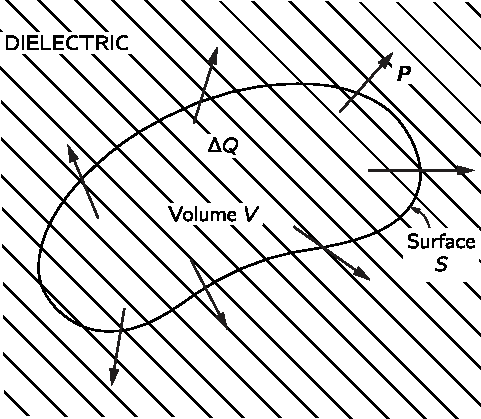
\includegraphics[width=0.5\linewidth]{fyz_fig711.pdf}
      \caption{
               (\cite[s.~707]{Feynman02})}
      \label{fyz:fig711}
    \end{figure}

    \begin{figure}[ht!] %\ref{fyz:fig712}
      \centering
      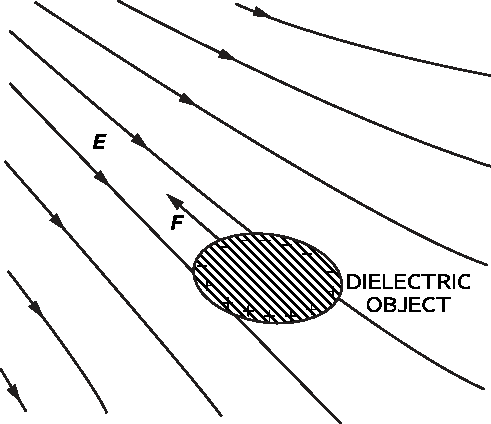
\includegraphics[width=0.5\linewidth]{fyz_fig712.pdf}
      \caption{
               (\cite[s.~707]{Feynman02})}
      \label{fyz:fig712}
    \end{figure}

    \begin{figure}[ht!] %\ref{fyz:fig713}
      \centering
      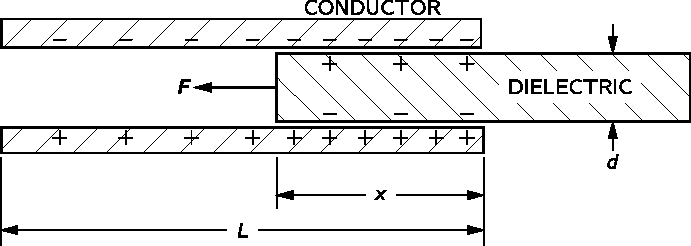
\includegraphics[width=0.5\linewidth]{fyz_fig713.pdf}
      \caption{
               (\cite[s.~707]{Feynman02})}
      \label{fyz:fig713}
    \end{figure}

\todo[inline]{Kapitola fey2ch10 je nedodělaná, obsahuje pouze obrázky}
%} %tikzset
%---------------------------------------------------------------------------------------------------
